\section{Monte Carlo Model of Deep Exclusive $\pi^{-}$ Production From The
  Neutron}

Our Monte Carlo studies require a
cross section model for an experimentally unexplored region of kinematics
at larger values of $Q^2$, $-t$ and $W$.
To briefly introduce the formalism, note that the scattering cross section
for $n(e,e^{\prime}\pi^{-})p$ in one-photon exchange is given by
equation~\ref{equation:cross-1}:

\begin{equation}
  \frac{d^{5} \sigma}{dE' d\Omega_{e'} d\Omega_{\pi}} = \Gamma_{V} \frac{d{^2}
    \sigma}{d\Omega_{\pi}}.
  \label{equation:cross-1}
\end{equation}

The virtual photon flux factor $\Gamma_{V}$ in Eq.~\ref{equation:cross-1} is
defined as:

\begin{equation}
  \Gamma_v=\frac{\alpha}{2\pi^2} \frac{E'}{E} \frac{K}{Q^2}\frac{1}{1-\epsilon},
  \label{equation:photon-flux-1}
\end{equation}
where $\alpha$ is the fine structure constant, $K$ is the energy of real photon
equal to the photon energy required to create a system with invariant mass
equal to $W$ and $\epsilon$ is the polarization of the virtual photon.

\begin{equation}
  K=(W^2-M_p^2)/(2 M_p)
  \label{equation:photon-flux-2}
\end{equation}

\begin{equation}
  \epsilon=\left(1+\frac{2 |\mathbf{q}|^2}{Q^2} \tan^2\frac{\theta_{e}}{2}
  \right)^{-1},
  \label{equation:photon-flux-3}
\end{equation}
where $\theta_{e}$ is the scattering angle of scattered electron. The two-fold
differential cross section $\frac{d{^2} \sigma}{d\Omega_{\pi}}$ in the lab
frame can be expressed in terms of the invariant cross section in center of
mass frame of photon and proton:

\begin{equation}
  \frac{d^2 \sigma}{d\Omega_\pi}= J \frac{d^2 \sigma}{dt d\phi},
  \label{equation:cross-2}
\end{equation}
where $J$ is the transformation of coordinates Jacobian from lab
$\Omega_{\pi}$ to $t$ and $\phi$ (CM). The invariant cross section of
Eq.~\ref{equation:cross-2} can be expressed in four terms. Two terms correspond
to the polarization states of the virtual photon (L and T) and two states
correspond to the interference of polarization states (LT and TT),

\begin{equation}
  2\pi \frac{d^2 \sigma}{dt d\phi} = \epsilon \frac{d\sigma_{\mathrm{L}}}{dt} +
  \frac{d\sigma_{\mathrm{T}}}{dt} + \sqrt{2\epsilon (\epsilon +1)}
  \frac{d\sigma_{\mathrm{LT}}}{dt} \cos{\phi} + \epsilon
  \frac{d\sigma_{\mathrm{TT}}}{dt} \cos{2 \phi}.
  \label{equation:cross-3}
\end{equation}

\subsection{Data Constraints}

Precise $L/T$ separated experimental data of exclusive electroproduction of
$\pi^{-}$ on $^2$H are available up to $Q^2=2.57$ GeV$^2$, $-t=0.350$
GeV$^2$ and $W=2.168$ GeV~\cite{gmhuber-2}. Precise $L/T$ separated
experimental data of exclusive electroproduction of $\pi^{+}$ on $^1$H are
available up to $Q^2=2.703$ GeV$^2$, $-t=0.365$ GeV$^2$ and $W=2.127$
GeV~\cite{Fpi2}. In Ref.~\cite{hallc-1} and Ref.~\cite{hallc-2}, separated
$\sigma_{L}$ and $\sigma_{T}$ are measured up to $Q^2=4.703$ GeV$^2$ and
$W=2.2$ GeV. CLAS experiment E99-105 measured the unseparated cross section at
$Q^2$ up to $4.35$ GeV$^2$ and $-t$ up to $4.5$ GeV$^2$~\cite{park}.  The
HERMES collaboration measured the unseparated cross section for $Q^2$=3.44
GeV$^2$ and 5.4 GeV$^2$~\cite{hermes} at $W$=4 GeV.

\subsection{Model for Higher $Q^2$ Kinematics}

The electroproduction of exclusive charged pions is best described by the VR
model~\cite{vr}. The VR model is a Regge model with a parameterization of deep
inelastic scattering amplitude to improve the description of $\sigma_{T}$. The
description of $\sigma_{L}$ is constrained by a fit to our Hall C data 
\cite{Fpi2}. In Fig.~\ref{fig:expvrfit}, we plotted the last six data
points of table $v$ of Ref.~\cite{gmhuber-2}, our parameterization and VR model
points for exactly same values of $Q^2$, $-t$ and $W$. It shows the comparison
of the same points of $\sigma_{L,T,LT,TT}$ vs. $Q^{2}$.

\begin{figure}[!hbt]
    \centering
    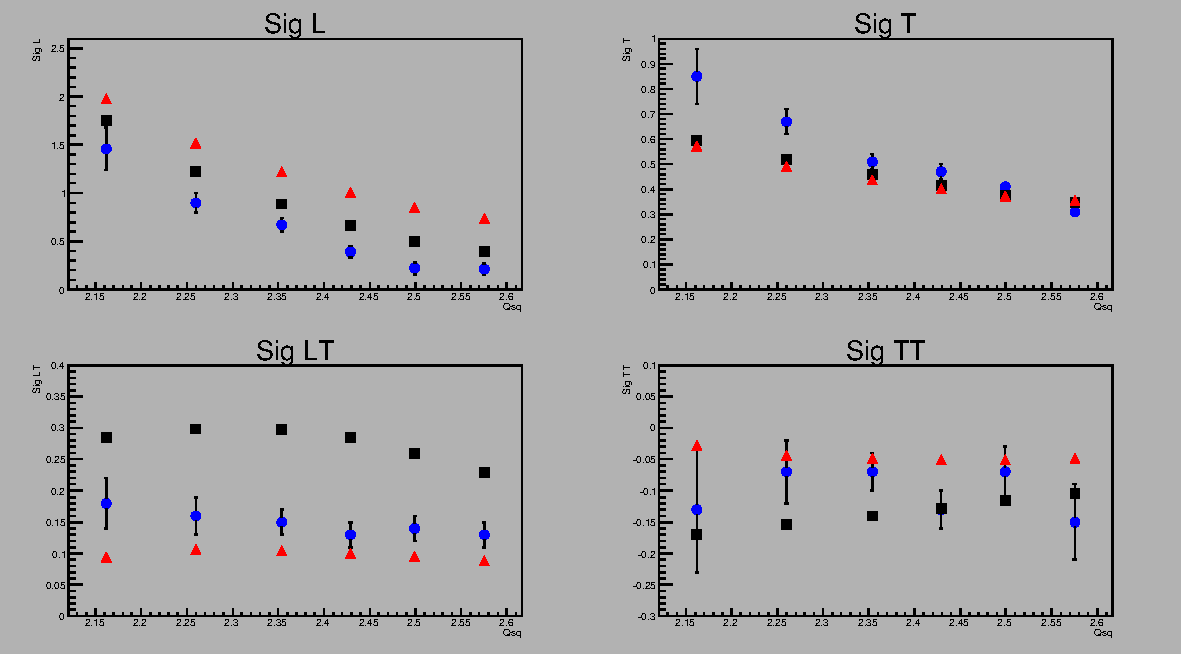
\includegraphics[width=6.0in,height=2.4in]{./figures/pimsigma_qsq.pdf}
    \caption{A $\pi^{-}$ electroproduction comparison for the last six points
      of table $v$ of Ref.~\cite{gmhuber-2}, the VR model and our
      parameterization values vs. $Q^{2}$. Experimental data is shown in blue
      circles, VR model is shown in red triangles and our parameterization is
      shown in black boxes. In each graph, the value of $-t$ is decreasing left
      to right from maximum value 0.35 GeV$^2$ to 0.15 GeV$^2$. Value of $W$
      also decreases left to right from 2.30 GeV to 2.17 GeV.}
    \label{fig:expvrfit}
\end{figure}

\subsection{Parameterization of $\sigma_{L}$, $\sigma_{T}$, $\sigma_{LT}$, 
$\&$ $\sigma_{TT}$}

For exclusive DEMP in SoLID, the kinematic region of interest for this
$\sigma_{L,T,LT,TT}$ parameterization is $Q^2$ from $4.5$ GeV$^2$ to 7.5
GeV$^2$, $-t$ from 0 GeV$^2$ to 1.0 GeV$^2$, and we set $W=3.0$ GeV. After
the parameterization of $\sigma_{L,T,LT,TT}$ for $-t$ and $Q^2$, we used the
same $W$ dependence given by Ref.~\cite{Fpi2}, which is $(W^2-M^2)^{-2}$
where $M$ is the proton mass. Our parameterization of all four cross sections
is given in Eq.~\ref{equation:l-fit} to Eq.~\ref{equation:tt-fit}:

\begin{equation}
        \sigma_{L} = \exp{(P_1(Q^2) + |t| * P^{\prime}_1(Q^2))} +
        \exp{(P_2(Q^2) + |t| * P^{\prime}_2(Q^2))}
     \label{equation:l-fit}
\end{equation}

\begin{equation}
        \sigma_{T} = \frac{\exp{(P_1(Q^2) + |t| *
            P^{\prime}_1(Q^2))}}{P_{1}(|t|)}
     \label{equation:t-fit}
\end{equation}

\begin{equation}
        \sigma_{LT} = P_{5}(t(Q^2))        
     \label{equation:lt-fit}
\end{equation}

\begin{equation}
        \sigma_{TT} = P_{5}(t(Q^2)),        
     \label{equation:tt-fit}
\end{equation}
where the parameters $P_{i}$ are polynomial functions of $i$th order. Each
coefficient ($P_{i}$) of fifth order equations Eq.~\ref{equation:lt-fit} and
Eq.~\ref{equation:tt-fit} is a further second order polynomial of $Q^2$. Deep
exclusive $\pi^{-}$ events are generated using a C++ code. The quality of
parameterization is checked by plotting the parameterization functions of
$\sigma_{L,T,LT,TT}$ versus the VR model as shown in Fig.~\ref{fig:sigall}.

\begin{figure}[!hbt]
    \centering
    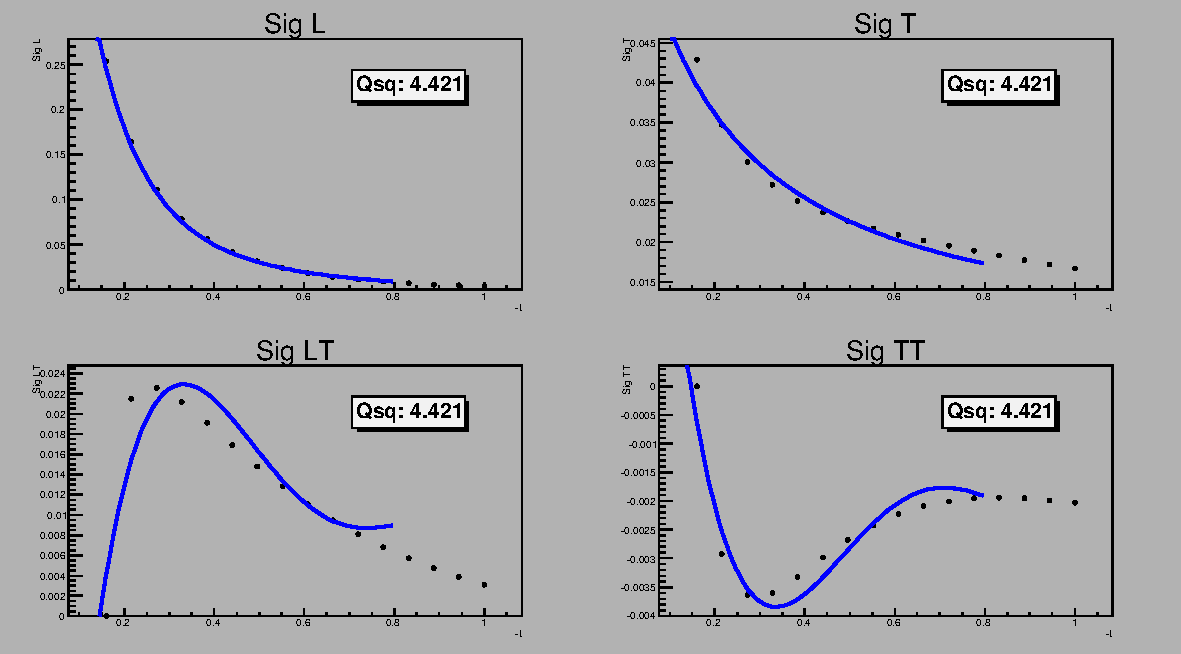
\includegraphics[width=6.0in,height=2.4in]{./figures/pimFit.pdf}
    \caption{A comparison of parameterized $\sigma_{L,T,LT,TT}$ and VR model
      values at $Q^2$=4.421~GeV$^2$ and $W=3.0$~GeV.  Black points are VR
      model values and the blue line is the parameterized $\sigma_{L,T,LT,TT}$
      given by equations Eq.~\ref{equation:l-fit} to
      Eq.~\ref{equation:tt-fit}.}
    \label{fig:sigall}
\end{figure}

\subsection{Single Spin Asymmetry (SSA) $\bf{A_{L}^{\perp}}$ }

It is shown in Ref.~\cite{Fr99} that the generalized parton distribution
($\tilde{E}$) can be probed by measuring the single spin asymmetry $(SSA)$. The
SSA is defined in Eq.~\ref{equation:ssa}
\begin{equation}
  \bf{A_{L}^{\perp}} =
  \frac{\int^{\pi}_{0}d\beta\frac{d\sigma_{L}^{\pi^{-}}}{d\beta} -
    \int^{2\pi}_{\pi}d\beta\frac{d\sigma_{L}^{\pi^{-}}}{d\beta} }
       {\int^{2\pi}_{0}d\beta\frac{d\sigma_{L}^{\pi^{-}}}{d\beta}},
     \label{equation:ssa}
\end{equation}
where $\beta$ is the angle between
the transversely polarized target vector and the reaction plane, and
$\sigma_{L}^{\pi^{-}}$ is the exclusive $\pi^{-}$ cross section for
longitudinal virtual photons.

We parameterized the single spin asymmetry using the model of Ref.~\cite{Fr00}
at $x=0.1$ and $x=0.3$, as given in Eq.~\ref{equation:asy-fit}
\begin{equation}
        \bf{A_{L}^{\perp}} = \left\{
        \begin{array}{rl}
        A_{0} \left[ 1 - \exp^{ [ -\lambda \times ( t - t_{min} ) ] } \right] &
        \text{if } t \ge t_{min}, \\ 0 & \text{if } t < t_{min}.
        \end{array} \right.
     \label{equation:asy-fit}
\end{equation}
The $SSA$ parameterization is compared to the model of Ref.~\cite{Fr00} in
Fig.~\ref{fig:asym-1}.

\begin{figure}[!hbt]
    \centering
    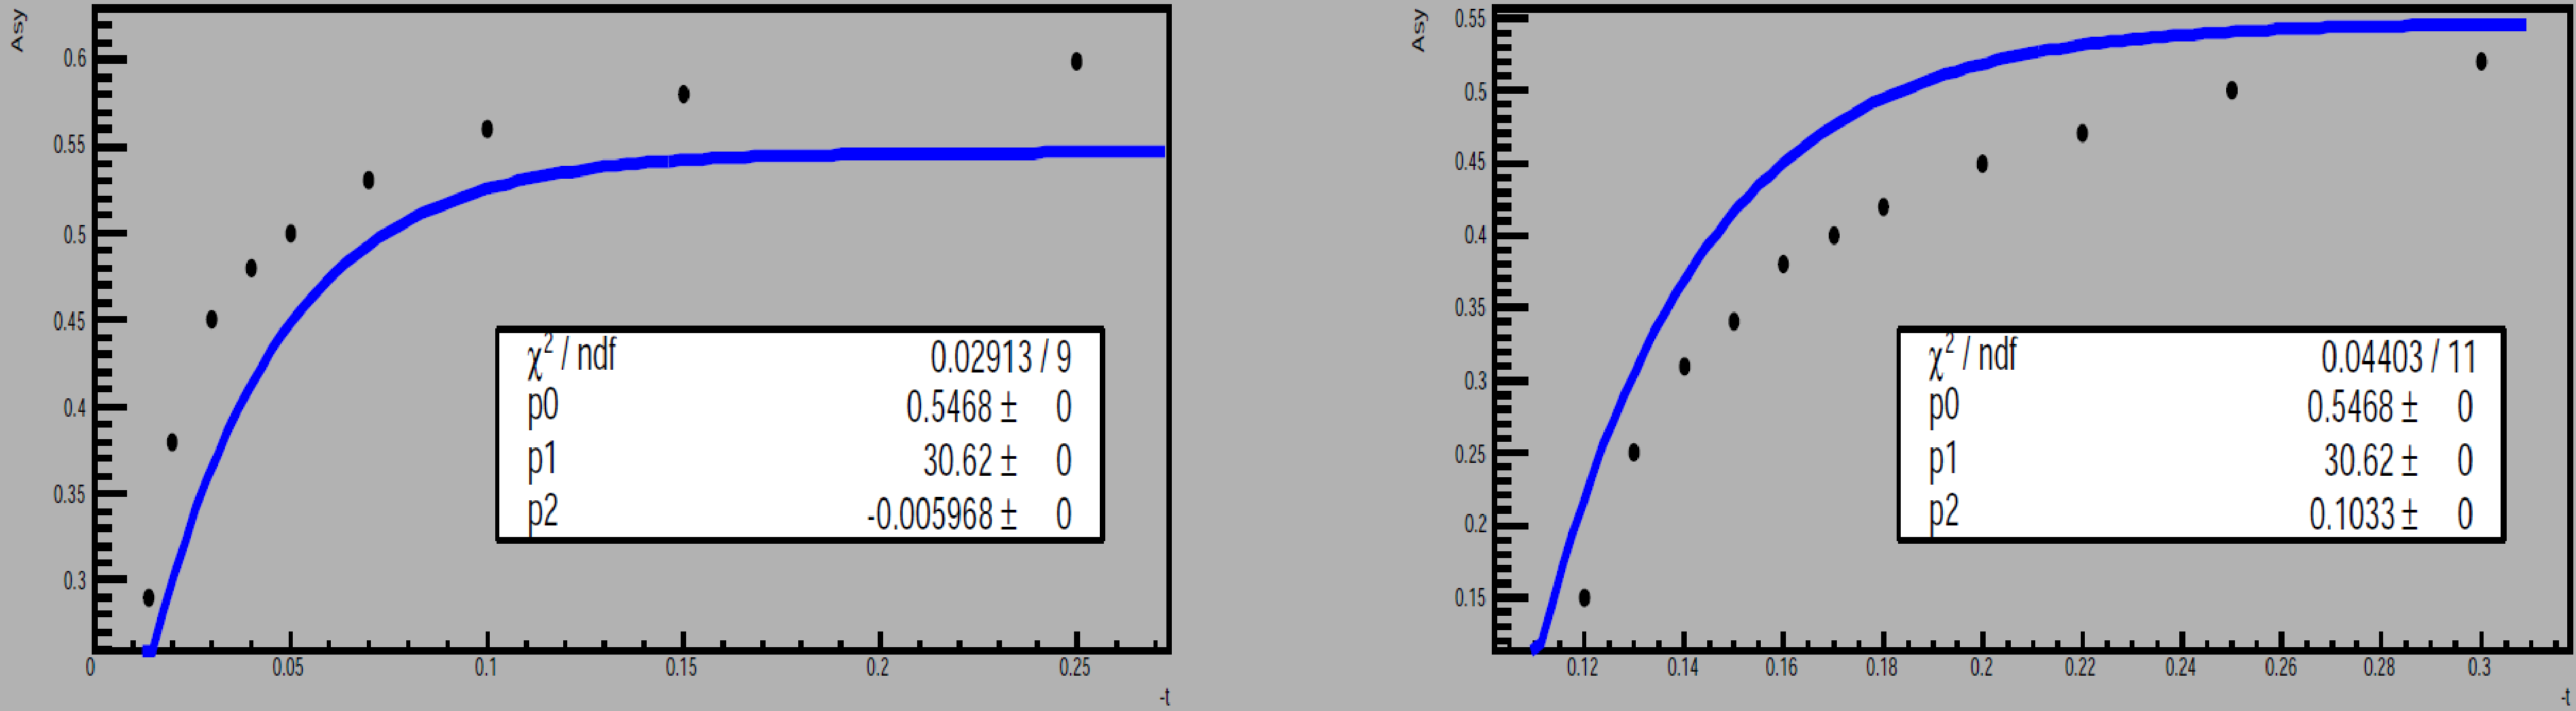
\includegraphics[width=6.0in,height=1.5in]{./figures/asym_3.pdf}
    \caption{Parameterization of single spin asymmetry $\bf{A_{L}^{\perp}}$
      vs. $-t$ at $x=0.1$ (left) and $x=0.3$ (right), where the points are from
      the model defined in Ref.~\cite{Fr00} and blue line is our
      parameterization function.}
    \label{fig:asym-1}
\end{figure}
